\documentclass{beamer}
\usetheme{Madrid}

\usepackage{amsmath, amssymb, amsthm}
\usepackage{graphicx}
\usepackage{listings}
\usepackage{gensymb}
\usepackage[utf8]{inputenc}
\usepackage{hyperref}
\usepackage{gvv}

\begin{document}

\title{ASSIGNMENT11.15\_13Q}
\author{EE22BTECH11219 - Rada Sai Sujan$^{}$% <-this % stops a space
}
\frame{\titlepage}

\begin{frame}
\frametitle{Question}
Given below are some functions of x and t to 
represent the displacement (transverse
or longitudinal) of an elastic wave. State which of these represents \brak i travelling
wave, \brak {ii} a stationary wave or \brak {iii} none at all: \\
\begin{enumerate}
\item $y = 2\cos \brak{3x} \sin \brak{10t}$
\item $y=2\sqrt{x-vt}$
\item $y = 3\sin \brak{5x - 0.5t} + 4\cos \brak{5x - 0.5t}$
\item $y = \cos x \sin t + \cos 2x \sin 2t$
\end{enumerate}
\end{frame}

\begin{frame}{allowframebreaks}
\frametitle{Solution: Theory}
\begin{tabular}{|p{2cm}|p{6cm}|}
    \hline
    PARAMETER & DESCRIPTION \\ \hline
    $G_c$ & Proportional controller's transfer function \\ \hline
    $G_f$ & Valve transfer function \\ \hline
    $G_p$ & Process transfer function   \\ \hline
    $G_M$ & Measurement transfer function \\ \hline 
    $G\brak{s}$ & Open loop transfer function \\ \hline
    $T\brak{s}$ & Transfer function of system \\ \hline
\end{tabular}

\end{frame}

\begin{frame}
\frametitle{Theory}
Let us assume an equation:
\begin{align}
y=A(x)\cos \brak{\omega t+\phi\brak {x}}
\end{align}
\end{frame}

\begin{frame}
\frametitle{Theory}
\begin{table}[htbp]
    \centering
    \def\arraystretch{1.5}
    \begin{tabular}{|p{4cm}|p{4cm}|}
    \hline
STATIONARY WAVE CONDITION & TRAVELLING WAVE CONDITION \\ \hline
        \brak 1 $A(x)$ should be a function of position x, and it can be expressed as $A(x)=A_{0}cos(\omega t+\alpha)$ where $A_{0}$ is a constant, $k$ is the wavenumber, $x$ is the position and $\alpha$ is a phase constant. & 
        \brak 1 $A(x)$ should be a constant, and it can be expressed as $A(x)=A_{0}$ where $A_{0}$ is a constant number. \\ \hline

        \brak 2 $\phi (x)$ can be expressed as $\phi (x)=c$ where c is a constant. &
        \brak 2 $\phi (x)$ is a linear expression in x or $\phi (x)=kx+\theta$ where k is the wavenumber and $\theta$ is the phaseconstant. \\ \hline
\end{tabular}
    \caption{Travelling wave $vs$ Stationary wave}
    \label{tab:table1}
\end{table}

\end{frame}

\begin{frame}
\frametitle{Graph}
\begin{figure}[ht]
                        \centering
                        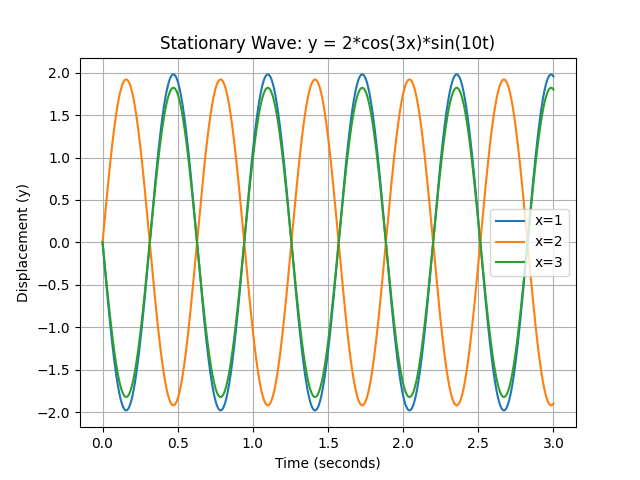
\includegraphics[width=\columnwidth]{figs/a.png}
                        \caption{DIPLACEMENT $vs$ TIME-graph1}
                        \label{fig:1}
\end{figure}
\end{frame}

\begin{frame}
\frametitle{Graph}
\begin{figure}[ht]
                            \centering
                            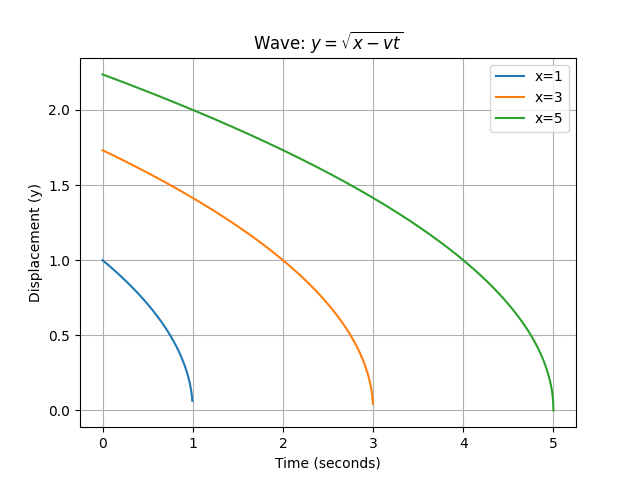
\includegraphics[width=\columnwidth]{figs/b.png}
                            \caption{DIPLACEMENT $vs$ TIME-graph2}
                            \label{fig:2}
\end{figure}   
\end{frame}

\begin{frame}
\frametitle{Graph}
\begin{figure}[ht]
                             \centering
                             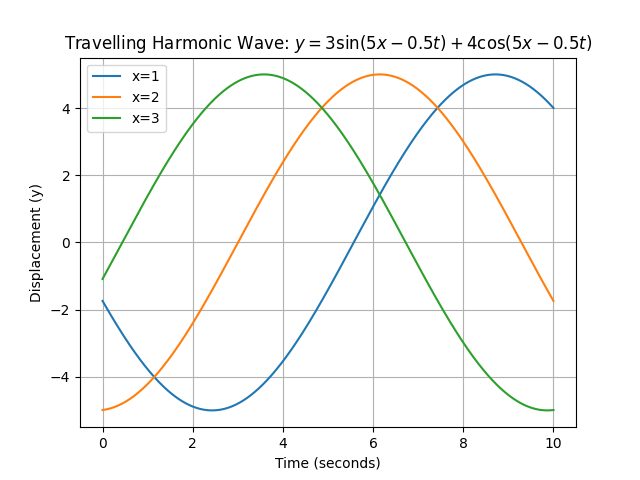
\includegraphics[width=\columnwidth]{figs/c.png}
                             \caption{DIPLACEMENT $vs$ TIME-graph3}
                             \label{fig:3}
\end{figure}
\end{frame}

\begin{frame}
\frametitle{Graph}
\begin{figure}[ht]
                            \centering
                            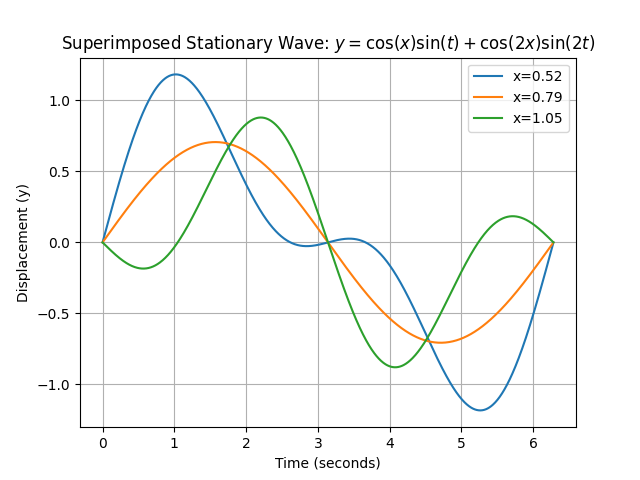
\includegraphics[width=\columnwidth]{figs/d.png}
                            \caption{DIPLACEMENT $vs$ TIME-graph4}
                            \label{fig:4}
\end{figure}
\end{frame}

\begin{frame}
\frametitle{Theory}
\figref{fig:1} and \figref{fig:3} are self explanatory for stationary and travelling waves.
\figref{fig:2} and \figref{fig:4} are neither stationary nor travelling waves. 
\end{frame}

\begin{frame}
\frametitle{Code}
\begin{figure}[ht]
                        \centering
                        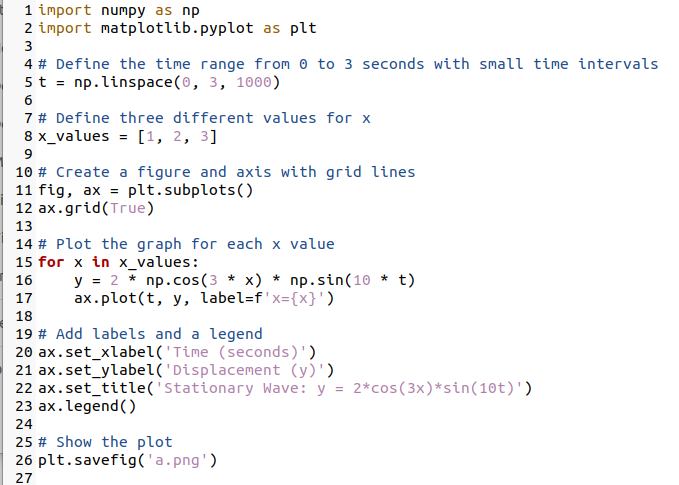
\includegraphics[width=\columnwidth]{figs/1.png}
                        \label{fig:1.1}
\end{figure}
\end{frame}

\begin{frame}
\frametitle{Code}
\begin{figure}[ht]
                        \centering
                        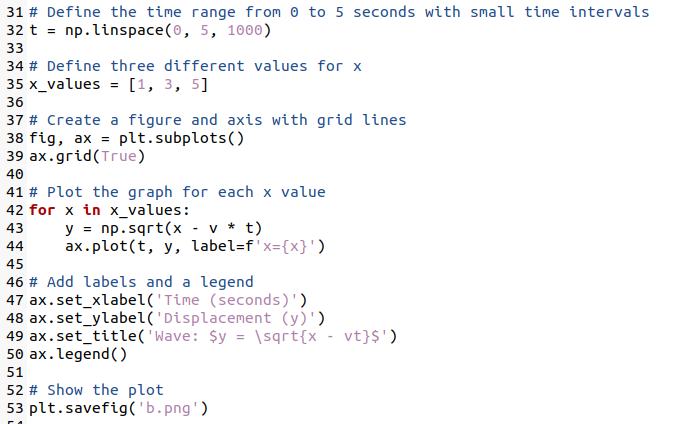
\includegraphics[width=\columnwidth]{figs/2.png}
                        \label{fig:1.2}
\end{figure}
\end{frame}

\begin{frame}
\frametitle{Code}
\begin{figure}[ht]
                        \centering
                        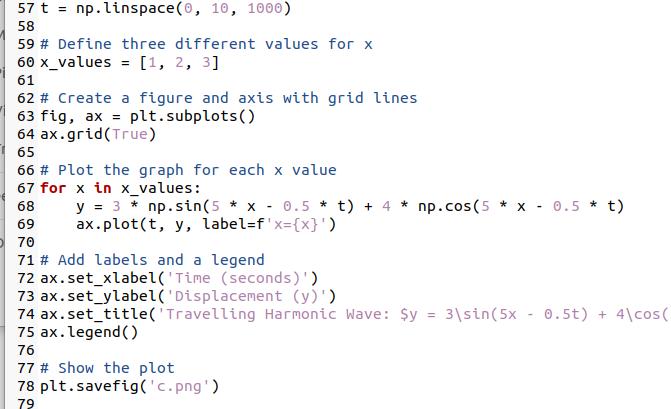
\includegraphics[width=\columnwidth]{figs/3.png}
                        \label{fig:1.3}
\end{figure}
\end{frame}

\begin{frame}
\frametitle{Code}
\begin{figure}[ht]
                        \centering
                        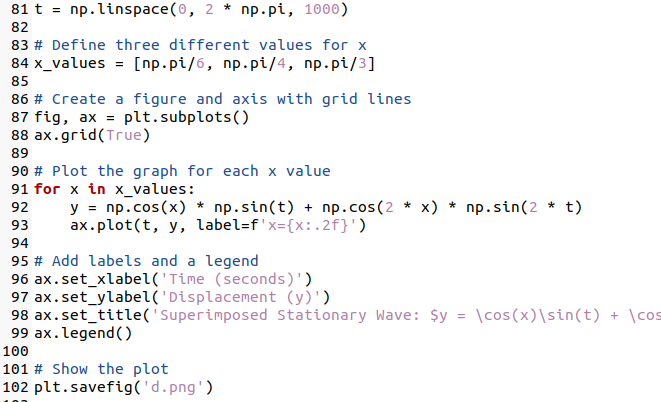
\includegraphics[width=\columnwidth]{figs/4.png}
                        \label{fig:1.3}
\end{figure}
\end{frame}
\end{document}
